\documentclass{article}
\usepackage{graphicx}
\usepackage{hyperref}
\graphicspath{ {../images/} }
\title{Project 3 Stat 159}
\author{Austin Carango, Youngshin Kim, Alexander Lee, Mandy Zhang}
\usepackage{Sweave}
\begin{document}
\Sconcordance{concordance:parent.tex:/Users/AustinCarango/stat159/stat159-fall2016-project3/report/parent.Rnw:%
1 6 1 1 0 3 1}
\Sconcordance{concordance:parent.tex:/Users/AustinCarango/stat159/stat159-fall2016-project3/report/sections/00-abstract.Rnw:ofs 11:%
1 4 1}
\Sconcordance{concordance:parent.tex:/Users/AustinCarango/stat159/stat159-fall2016-project3/report/parent.Rnw:ofs 16:%
12}
\Sconcordance{concordance:parent.tex:/Users/AustinCarango/stat159/stat159-fall2016-project3/report/sections/01-introduction.Rnw:ofs 17:%
1 7 1}
\Sconcordance{concordance:parent.tex:/Users/AustinCarango/stat159/stat159-fall2016-project3/report/parent.Rnw:ofs 25:%
14}
\Sconcordance{concordance:parent.tex:/Users/AustinCarango/stat159/stat159-fall2016-project3/report/sections/02-data.Rnw:ofs 26:%
1 31 1}
\Sconcordance{concordance:parent.tex:/Users/AustinCarango/stat159/stat159-fall2016-project3/report/parent.Rnw:ofs 58:%
16}
\Sconcordance{concordance:parent.tex:/Users/AustinCarango/stat159/stat159-fall2016-project3/report/sections/03-methods.Rnw:ofs 59:%
1 4 1}
\Sconcordance{concordance:parent.tex:/Users/AustinCarango/stat159/stat159-fall2016-project3/report/parent.Rnw:ofs 64:%
18}
\Sconcordance{concordance:parent.tex:/Users/AustinCarango/stat159/stat159-fall2016-project3/report/sections/04-analysis.Rnw:ofs 65:%
1 5 1 1 2 1 0 1 2 1 1 1 2 1 1 1 2 3 0 1 2 4 1 1 3 1 0 3 2 1 1 1 2 4 0 1 %
3 4 1 1 3 1 0 1 2 1 1 2 2 1 3 1 0 1 2 4 0 1 3 4 1 1 3 1 0 1 2 1 1 2 2 1 %
1 1 2 1 1 2 2 4 0 1 3 1 1}
\Sconcordance{concordance:parent.tex:/Users/AustinCarango/stat159/stat159-fall2016-project3/report/parent.Rnw:ofs 137:%
20}
\Sconcordance{concordance:parent.tex:/Users/AustinCarango/stat159/stat159-fall2016-project3/report/sections/05-results.Rnw:ofs 138:%
1 3 1 1 10 25 0 1 2 4 1 1 7 43 0 1 2 4 1 1 15 42 0 1 2 4 1 1 8 16 0 1 2 %
1 1}
\Sconcordance{concordance:parent.tex:/Users/AustinCarango/stat159/stat159-fall2016-project3/report/parent.Rnw:ofs 289:%
22}
\Sconcordance{concordance:parent.tex:/Users/AustinCarango/stat159/stat159-fall2016-project3/report/sections/06-conclusion.Rnw:ofs 290:%
1 4 1}
\Sconcordance{concordance:parent.tex:/Users/AustinCarango/stat159/stat159-fall2016-project3/report/parent.Rnw:ofs 295:%
24 2 1}

\maketitle

\section{Abstract}

The goal of this project is to create a predictive modeling process for the College Scorecard dataset from the perspective of a consultant whose client is a group of administrators trying to make their school more competetive. The data contains information pertaining to the "cost and value of institutions accross the country" and can be found at \url{https://collegescorecard.ed.gov/data/}.



\section{Introduction}

Given the College Scorecard data, which contains a variety of information including academics, demographics, cost, and earnings for thousands of colleges in America, how can a group of administrators increase the competitiveness of their school?

To answer this, we look at 4 different regression methods, including OLS, PLSR, LASSO and Random Tree. Each of these methods will be individually discussed and applied to the College Scorecard data. Then, each model will be compared and recommondations for the administrators will be given based off the results of the regressions.

We will attempt to model earnings of graduates as a function of 33 other variables, which will be discussed in detail in the next section. 


\section{Data}

The dataset used in this project is called Most-Recent-Cohorts-All-Data-Elements.csv, and can be found at \url{https://collegescorecard.ed.gov/data/}. This particular subset contains only the most recent data, which we are interested in because we want to predict future outcomes. The raw data contains 7703 observations of 1743 variables, each observation being a college.

Before performing analysis of any kind this data was cleaned and scaled. This involved first picking out only private colleges from the data and selecting a subset of variables of interest. Then, rows and columns for which there were an abundance of NA values were deleted. Then, any remaining NA values were imputed with column means. Finally, the data was mean centered and standardized. This resulted in the dataset we will analyze, final.csv.

This file contains 34 variables. The response variable is called Earning, renamed from MN\_EARN\_WNE\_P10, and indicates the mean earnings of federally aided students 10 years after enrolling. We take this to be a good indicator of competitiveness, as high mean earnings after graduation are desirable. The 33 explanatory variables are as follows:

\textbullet\ HIGHDEG is the highest level of degree awarded by the institution, in descending order of graduate degree/certificate, bachelor's, associate's, and certificate.

\textbullet\ TUITFTE is the net tuition revenue per full-time student

\textbullet\ SATVR25/75, SATMT25/75, ACTEN25/75, and ACTMT25/75 are the 25th and 75th percentile scores for enrolled students in the English and math sections of the SAT and ACT.

\textbullet\ COSTT4\_A is the average cost of attendance, tuition and fees

\textbullet\ NPT4\_PRIV is the average net price of attending.

\textbullet\ UGDS is the number of undergraduates enrolled in the fall.

\textbullet\ UGDS\_WHITE, UGDS\_BLACK, UGDS\_HISP, UGDS\_ASIAN, UGDS\_AIAN, UGDS\_NHPI, UGDS\_2MOR, UGDS\_NRA, UGDS\_UNKN, respectively indicate the number of white, black, Hispanic, Asian, American Indian/Alaska Native, Native Hawaiian/Pacific Islander, bi or multiracial, non-resident alien, and unknown race students.

\textbullet\ MARRIED, DEPENDENT and FIRST\_GEN indicate the share of married, dependent and first generation students.

\textbullet\ PCTFLOAN indicates the share of students who recieved federal loans.

\textbullet\ PCTPELL indicates the share of students who recieved Pell Grants.

\textbullet\ C100\_4 and C150\_4 are the graduation rates for full-time, first-time students within 100 or 150 percent of expected completion time.

\textbullet\ GT\_25K\_P10 is the fraction of students earning over 25 thousand dollars per year 10 years after enrolling.


\section{Methodology}

We analyze the data using four regression methods: original least squares (OLS), partial least squares (PLSR), lasso, and random forest. The OLS method simply creates a linear model based on our 34 predictive variables which minimizes the residual sum of squares. PLSR is a dimension reduction method, which is useful when variables are correlated with each other; since it is unknown if our varaibles are correlated, we run a PLSR to generate a model and compare it to the others. Lasso is a shrinkage method, aiming to find a model with the smallest lambda. The random forest method makes predictions using regression trees, which split the data into smaller and smaller subsets such that the residual sum of squares is reduced; the random forest model builds trees based on bootstrapped training samples, which decorrelates the trees, making them more reliable. This is done via the "caret" package, which simplifies regression training.



\section{Analysis}

In this section we show the processes used in each of the four regression methods by displaying the code used. Diagnostic/validation plots are also displayed for each regression.

\subsection{OLS}

\begin{Schunk}
\begin{Sinput}
> set.seed(159)
> edu = read.csv('../data/final.csv', stringsAsFactors = FALSE)
> edu = edu[, -c(1)]
> ols = lm(Earning~., data = edu)
> ols_summary = summary(ols)
> save(ols, file = '../data/ols.RData')
\end{Sinput}
\end{Schunk}

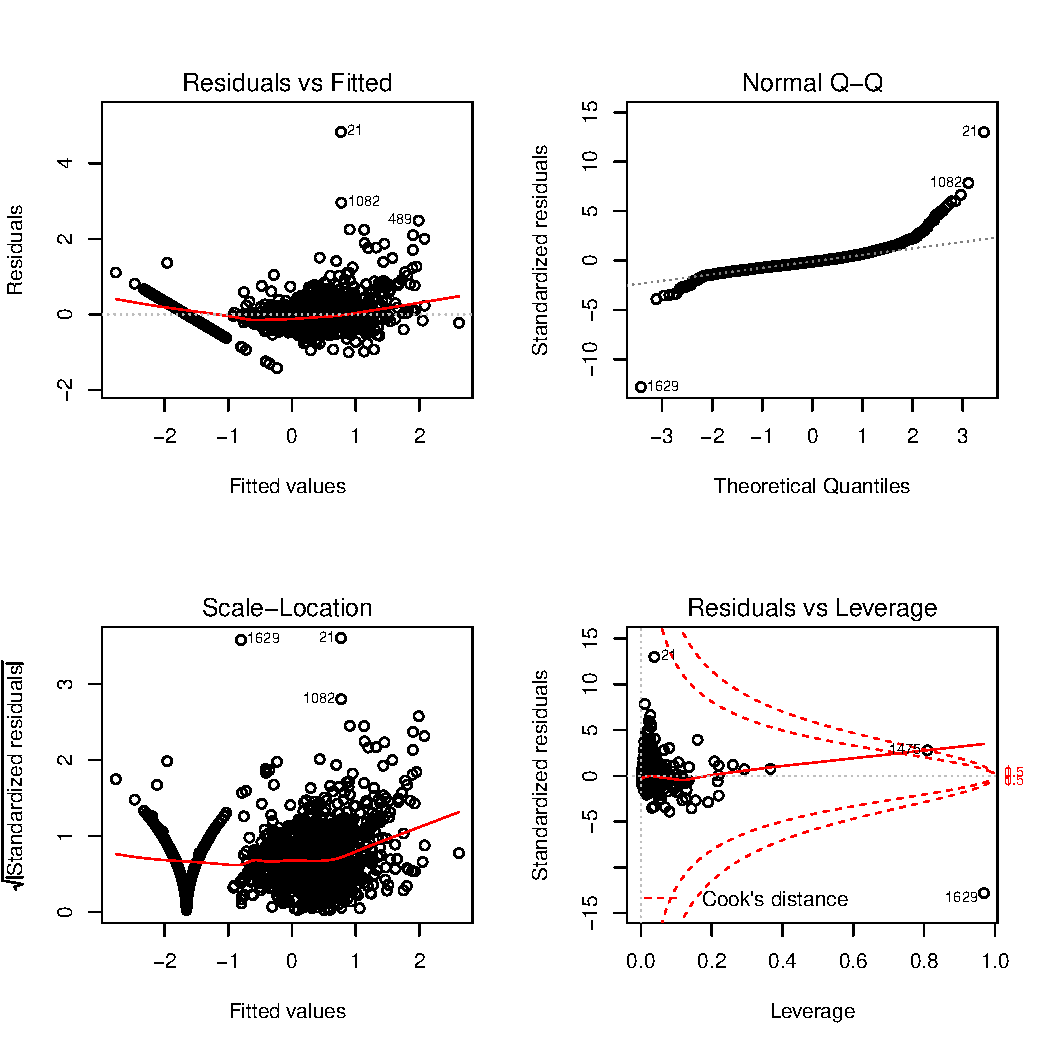
\includegraphics{ols.pdf}

\subsection{PLSR}

\begin{Schunk}
\begin{Sinput}
> library(pls)
> set.seed(159)
> plsr = plsr(Earning~., data = edu, validation ="CV", scale = FALSE,standardize = FALSE)
> plsr_coef = plsr$coefficients[,1,which.min(plsr$validation$PRESS)]
> plsr_coef
> save(plsr, file = '../data/plsr.RData')
> 
\end{Sinput}
\end{Schunk}

\includegraphics{plsr.pdf}

\subsection{Lasso}

\begin{Schunk}
\begin{Sinput}
> library(glmnet)
> edu = read.csv('../data/final.csv', stringsAsFactors = FALSE)
> edu = edu[, -c(1)]
> grid = 10^seq(10, -2, length=100)
> set.seed(159)
> lasso = cv.glmnet(as.matrix(edu[,c(1:33)]), as.matrix(edu[,34]), intercept = FALSE,
+                    standardize = FALSE, lambda = grid, alpha = 1)
> save(lasso, file = '../data/lasso.RData')
> 
\end{Sinput}
\end{Schunk}

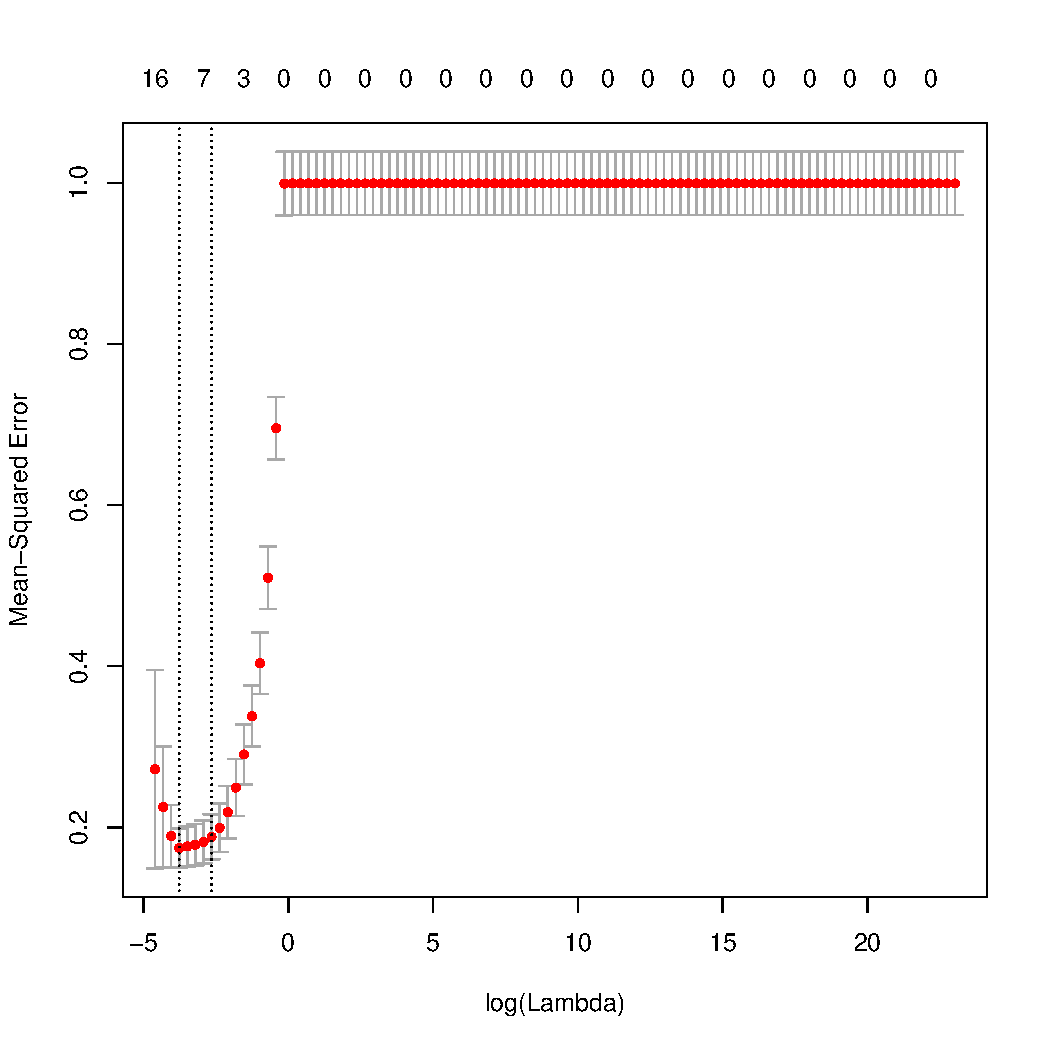
\includegraphics{lasso.pdf}

\subsection{Random Forest}

\begin{Schunk}
\begin{Sinput}
> library(caret)
> edu = read.csv('../data/final.csv', stringsAsFactors = FALSE)
> edu = edu[, -c(1)]
> train_index = sample(1:1636, 1336)
> train = edu[train_index,]
> test = edu[-train_index,]
> fitControl = trainControl(method = "repeatedcv", number = 10)
> model.rf = train(Earning ~ ., data = train, method = 'rf', trControl = fitControl)
> importance(model.rf$finalModel)
> save(model.rf, file = '../data/randomforest.RData')
> 
\end{Sinput}
\end{Schunk}

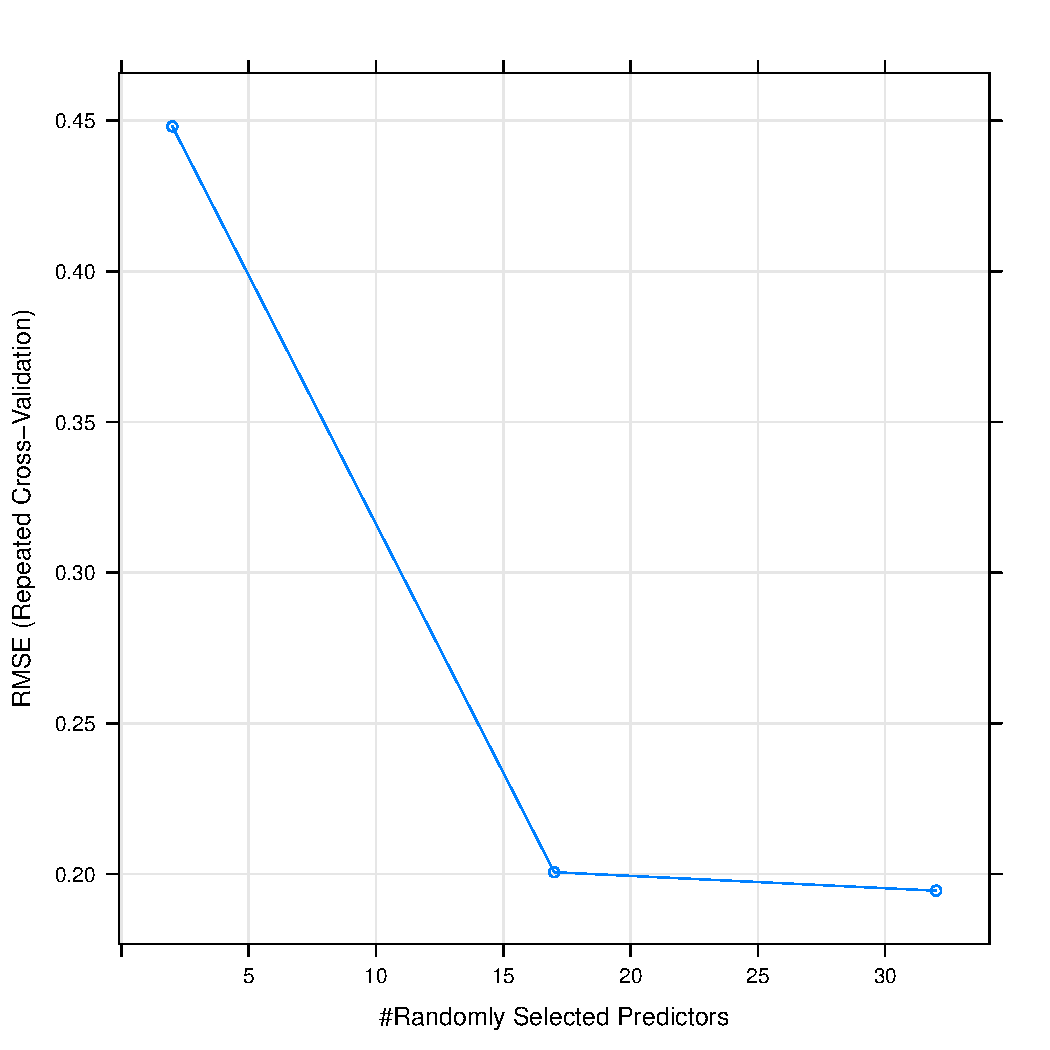
\includegraphics{randomforest.pdf}

\section{Results}

\subsection{OLS}

% latex table generated in R 3.2.3 by xtable 1.8-2 package
% Mon Dec  5 00:16:11 2016
\begin{table}[ht]
\centering
\begin{tabular}{rrr}
  \hline
 & Estimate & Pr...t.. \\ 
  \hline
TUITFTE & 0.02 & 0.01 \\ 
  SATVR25 & 0.55 & 0.00 \\ 
  SATVR75 & -0.62 & 0.00 \\ 
  SATMT25 & 0.46 & 0.00 \\ 
  ACTEN25 & 0.34 & 0.00 \\ 
  ACTEN75 & -0.49 & 0.00 \\ 
  ACTMT25 & 0.42 & 0.00 \\ 
  ACTMT75 & -0.30 & 0.02 \\ 
  COSTT4\_A & 0.17 & 0.00 \\ 
  NPT4\_PRIV & -0.09 & 0.00 \\ 
  UGDS & 0.07 & 0.00 \\ 
  DEPENDENT & -0.03 & 0.02 \\ 
  PCTFLOAN & 0.06 & 0.00 \\ 
  PCTPELL & -0.14 & 0.00 \\ 
  GT\_25K\_P10 & 0.81 & 0.00 \\ 
   \hline
\end{tabular}
\caption{OLS Significant Coefficients} 
\end{table}
From these results we can see that the primary predictors of earning are SAT and ACT scores. Other significant variables are tuition, annual cost of attendance, the average net price of attendance, the number of undergraduates, dependence, the borrowing rate, and reception of a Pell grant.

\subsection{PLSR}

% latex table generated in R 3.2.3 by xtable 1.8-2 package
% Mon Dec  5 00:16:11 2016
\begin{table}[ht]
\centering
\begin{tabular}{rlr}
  \hline
 & variable & coefficient \\ 
  \hline
1 & HIGHDEG & -0.00 \\ 
  2 & TUITFTE & 0.03 \\ 
  3 & SATVR25 & 0.03 \\ 
  4 & SATVR75 & -0.01 \\ 
  5 & SATMT25 & 0.06 \\ 
  6 & SATMT75 & 0.01 \\ 
  7 & ACTEN25 & 0.01 \\ 
  8 & ACTEN75 & -0.05 \\ 
  9 & ACTMT25 & 0.02 \\ 
  10 & ACTMT75 & -0.03 \\ 
  11 & COSTT4\_A & 0.09 \\ 
  12 & NPT4\_PRIV & -0.08 \\ 
  13 & UGDS & 0.09 \\ 
  14 & UGDS\_MEN & 0.04 \\ 
  15 & UGDS\_WOMEN & -0.03 \\ 
  16 & UGDS\_WHITE & -0.01 \\ 
  17 & UGDS\_BLACK & -0.00 \\ 
  18 & UGDS\_HISP & -0.00 \\ 
  19 & UGDS\_ASIAN & 0.14 \\ 
  20 & UGDS\_AIAN & -0.01 \\ 
  21 & UGDS\_NHPI & -0.00 \\ 
  22 & UGDS\_2MOR & 0.00 \\ 
  23 & UGDS\_NRA & -0.02 \\ 
  24 & UGDS\_UNKN & -0.02 \\ 
  25 & MARRIED & -0.04 \\ 
  26 & DEPENDENT & -0.03 \\ 
  27 & FIRST\_GEN & 0.05 \\ 
  28 & PCTFLOAN & 0.02 \\ 
  29 & PCTPELL & -0.16 \\ 
  30 & COSTT4\_A.1 & 0.09 \\ 
  31 & C100\_4 & -0.03 \\ 
  32 & C150\_4 & -0.04 \\ 
  33 & GT\_25K\_P10 & 0.80 \\ 
   \hline
\end{tabular}
\caption{PLSR Coefficients} 
\end{table}
The coefficients of the PLSR model with the lowest lambda value. Of particular note are the number of Asian undergraduates (the highest value) and the number of students receiving a Pell grant (the lowest value).

\subsection{lasso}

% latex table generated in R 3.2.3 by xtable 1.8-2 package
% Mon Dec  5 00:16:12 2016
\begin{table}[ht]
\centering
\begin{tabular}{rlr}
  \hline
 & variable & coefficient \\ 
  \hline
1 & TUITFTE & 0.01 \\ 
  2 & SATVR25 & 0.00 \\ 
  3 & SATVR75 & 0.00 \\ 
  4 & SATMT25 & 0.05 \\ 
  5 & SATMT75 & 0.00 \\ 
  6 & ACTEN25 & 0.00 \\ 
  7 & ACTEN75 & 0.00 \\ 
  8 & ACTMT25 & 0.00 \\ 
  9 & ACTMT75 & 0.00 \\ 
  10 & COSTT4\_A & 0.08 \\ 
  11 & NPT4\_PRIV & 0.00 \\ 
  12 & UGDS & 0.07 \\ 
  13 & UGDS\_MEN & 0.00 \\ 
  14 & UGDS\_WOMEN & 0.00 \\ 
  15 & UGDS\_WHITE & 0.00 \\ 
  16 & UGDS\_BLACK & 0.00 \\ 
  17 & UGDS\_HISP & 0.00 \\ 
  18 & UGDS\_ASIAN & 0.12 \\ 
  19 & UGDS\_AIAN & 0.00 \\ 
  20 & UGDS\_NHPI & 0.00 \\ 
  21 & UGDS\_2MOR & 0.00 \\ 
  22 & UGDS\_NRA & 0.00 \\ 
  23 & UGDS\_UNKN & 0.00 \\ 
  24 & MARRIED & -0.01 \\ 
  25 & DEPENDENT & -0.01 \\ 
  26 & FIRST\_GEN & 0.00 \\ 
  27 & PCTFLOAN & 0.00 \\ 
  28 & PCTPELL & -0.13 \\ 
  29 & COSTT4\_A.1 & 0.00 \\ 
  30 & C100\_4 & 0.00 \\ 
  31 & C150\_4 & 0.00 \\ 
  32 & GT\_25K\_P10 & 0.76 \\ 
   \hline
\end{tabular}
\caption{Lasso Coefficients} 
\end{table}
The coefficients of the lasso regression model. The highest is the number of Asian undergraduates and the lowest is the number of students receiving a Pell grant.

\subsection{randomForest}

% latex table generated in R 3.2.3 by xtable 1.8-2 package
% Mon Dec  5 00:16:13 2016
\begin{table}[ht]
\centering
\begin{tabular}{rlr}
  \hline
 & variable & IncNodePurity \\ 
  \hline
1 & TUITFTE & 32.97 \\ 
  4 & SATMT25 & 9.60 \\ 
  15 & UGDS\_WHITE & 5.59 \\ 
  18 & UGDS\_ASIAN & 28.33 \\ 
  27 & PCTFLOAN & 9.84 \\ 
  32 & GT\_25K\_P10 & 1176.88 \\ 
   \hline
\end{tabular}
\caption{Relevant Variables from Random Forest} 
\end{table}
The variables with a higher IncNodePurity value were the significant ones, which had more of an effect predicting the earnings of a student. These variables are tuition, race (being white or Asian), and receiving a loan in college.

\section{Conclusion}

The models above tend to agree that tuition, SAT/ACT scores, total cost of attendance, the racial composition of the undergraduate classes, taking out a loan, and receiving a Pell grant. However, these variables may not be useful in the context of making changes to the campus's administration to increase competitiveness. To begin with, the fact that tuition predicts eventual earnings is clear: schools that require higher tuition levels are typically better schools academically, and thus it would be clear that attending a school with a higher tuition would lead to finding a higher-paying job in the future. It is not the case that increasing tuition at your college would necessarily lead to an increase in competitiveness. There is a similar argument for the cost of attendance, as tuition is included in that cost, and for taking out a loan, as students at universities that have higher tuition would typically have to take out loans in order to pay the amount. Of interest is the negative correlation between earnings later and receiving a Pell grant in college: the models agree that having a Pell grant predicts lower earnings later in life. 



\end{document}

